\documentclass{amsart}
\usepackage[dvipsnames]{xcolor}
\usepackage{tikz}
\newcommand*{\bigdots}{{\Large $\vdots$}}
\begin{document}
\begin{figure}
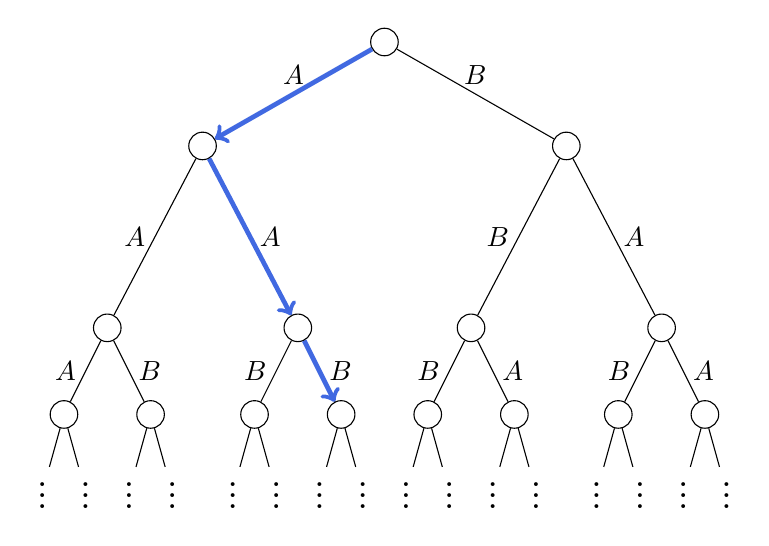
\begin{tikzpicture}
[
    scale = 1.1,
    level 1/.style={sibling distance=42mm, level distance = 1.2cm},
    level 2/.style={sibling distance=22mm, level distance = 2.1cm},
    level 3/.style={sibling distance = 10mm, level distance = 1cm},
    level 4/.style={sibling distance = 5mm, level distance = .9cm},
    ellip/.style={text height = 4mm},
    game/.style={circle, draw, minimum size = .35cm, fill = none},
    whole/.style={draw=black, very thick, inner sep = 25pt, text height = 0mm},
    sub/.style={dashed, draw=black, very thick, inner sep=15pt}, % Style for grouping
    ssub/.style={draw = black, very thick, inner sep = 3pt},
    arrow/.style={draw, ->, color = RoyalBlue, line width = 1.7pt},
]

% Draw the binary tree with an edge label
\node[game] (root) {}
	child {node[game](11) {}
		child {node[game] {}
			child {node[game] {}
				child {node[ellip] {\bigdots}}
				child {node[ellip] {\bigdots}}
			edge from parent node [left] {$A$}
				}
			child {node[game] {}
				child {node[ellip] {\bigdots}}
				child {node[ellip] {\bigdots}}
			edge from parent node [right] {$B$}
				}
	edge from parent node [left] {$A$}
			}
		child {node[game](22) {}
			child {node[game] {}
				child {node[ellip] {\bigdots}}
				child {node[ellip] {\bigdots}}
			edge from parent node [left] {$B$}
				}
			child {node[game](34) {}
				child {node[ellip] {\bigdots}}
				child {node[ellip] {\bigdots}}
			edge from parent node [right] {$B$}
				}
		edge from parent node [right] {$A$}
			}
	edge from parent node [above] {$A$}
	}
	child {node[game] {}
		child {node[game] {}
			child {node[game] {}
				child {node[ellip] {\bigdots}}
				child {node[ellip] {\bigdots}}
			edge from parent node [left] {$B$}
				}
			child {node[game] {}
				child {node[ellip] {\bigdots}}
				child {node[ellip] {\bigdots}}
			edge from parent node [right] {$A$}
				}
		edge from parent node [left] {$B$}
			}
		child {node[game] {}
			child {node[game] {}
				child {node[ellip] {\bigdots}}
				child {node[ellip] {\bigdots}}
			edge from parent node [left] {$B$}
				}
			child {node[game](s) {}
				child {node[ellip] {\bigdots}}
				child {node[ellip] {\bigdots}}
			edge from parent node [right] {$A$}
				}
		edge from parent node [right] {$A$}
			}
	edge from parent node [above] {$B$}
	};
	\draw[arrow] (root) -- (11);
	\draw[arrow] (11) -- (22);
	\draw[arrow] (22) -- (34);
\end{tikzpicture}
\caption{An infinite binary tree where two players, Aaron and Berren, compete head to head. Each edge is labelled $A$ with probability $p$ and $B$ with probability $1-p$. The two players take turns on which edge to traverse. If an edge with $B$ is ever traversed, Berren wins. Otherwise, Aaron wins. What is the infimum of the set of probabilities $p$ for which Aaron has a nonzero probability of winning?}
\end{figure}
\end{document}
